% Seq2seq bottleneck — TikZ source. Compiles to a tight standalone PDF
% (pdflatex figures/seq2seq-bottleneck.tex), which `book-scaffold build-figures`
% converts to public/figures/seq2seq-bottleneck.svg.
%
% Every encoder input x_1..x_n and every decoder output y_1..y_m communicates
% ONLY through the single fixed-size vector c = h_n: dimension d_s does not
% grow with n, so the map from inputs to contexts cannot stay injective for
% large n — the pigeonhole bottleneck (prop-seq2seq-fixed-vector-bottleneck).
\documentclass[tikz,border=3pt]{standalone}
\usepackage{amsmath}
\usepackage{amssymb}
\usepackage{tikz}
\usetikzlibrary{positioning,arrows.meta,calc}
\begin{document}
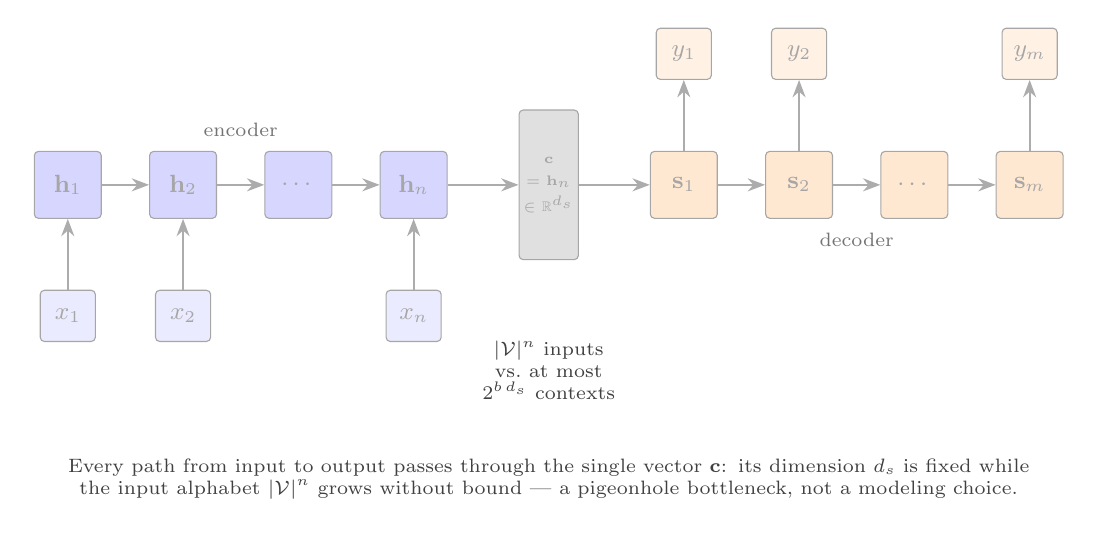
\begin{tikzpicture}[
    font=\small,
    state/.style={draw, gray!70, rounded corners=1.5pt, align=center,
                  minimum width=8.5mm, minimum height=8.5mm, inner sep=1pt},
    enc/.style={state, fill=blue!16},
    dec/.style={state, fill=orange!18},
    tokbox/.style={draw, gray!70, rounded corners=1.5pt, align=center,
                   minimum width=7mm, minimum height=6.5mm, inner sep=1pt},
    inbox/.style={tokbox, fill=blue!8},
    outbox/.style={tokbox, fill=orange!10},
    neck/.style={draw, gray!70, rounded corners=1.5pt, align=center,
                 fill=black!12, font=\tiny, inner sep=1.5pt,
                 minimum width=7mm, minimum height=19mm},
    op/.style={->, >={Stealth[length=2.2mm]}, gray!65, thick},
    rolelbl/.style={font=\scriptsize, text=black!55},
  ]
  % --- encoder chain (middle row, left half) ---
  \node[enc] (h1) {$\mathbf h_1$};
  \node[enc, right=6mm of h1] (h2) {$\mathbf h_2$};
  \node[enc, right=6mm of h2] (hdots) {$\cdots$};
  \node[enc, right=6mm of hdots] (hn) {$\mathbf h_n$};

  % --- bottleneck neck (center) ---
  \node[neck, right=9mm of hn] (c) {$\mathbf c$\\[2pt]$=\mathbf h_n$\\[2pt]$\in\mathbb R^{d_s}$};

  % --- decoder chain (middle row, right half) ---
  \node[dec, right=9mm of c] (s1) {$\mathbf s_1$};
  \node[dec, right=6mm of s1] (s2) {$\mathbf s_2$};
  \node[dec, right=6mm of s2] (sdots) {$\cdots$};
  \node[dec, right=6mm of sdots] (sm) {$\mathbf s_m$};

  % --- encoder inputs (below, feeding up) ---
  \node[inbox, below=9mm of h1] (x1) {$x_1$};
  \node[inbox, below=9mm of h2] (x2) {$x_2$};
  \node[inbox, below=9mm of hn] (xn) {$x_n$};

  % --- decoder outputs (above, read off) ---
  \node[outbox, above=9mm of s1] (y1) {$y_1$};
  \node[outbox, above=9mm of s2] (y2) {$y_2$};
  \node[outbox, above=9mm of sm] (ym) {$y_m$};

  % --- role labels (mirrored, in the otherwise-empty half of each side) ---
  \node[rolelbl] at ($(h1)!0.5!(hn)+(0,7mm)$) {encoder};
  \node[rolelbl] at ($(s1)!0.5!(sm)+(0,-7mm)$) {decoder};

  % --- arrows: inputs feed the encoder chain ---
  \draw[op] (x1) -- (h1);
  \draw[op] (x2) -- (h2);
  \draw[op] (xn) -- (hn);

  % --- arrows: encoder recurrence ---
  \draw[op] (h1) -- (h2);
  \draw[op] (h2) -- (hdots);
  \draw[op] (hdots) -- (hn);

  % --- arrows: the ONLY encoder-decoder channel ---
  \draw[op] (hn) -- (c);
  \draw[op] (c) -- (s1);

  % --- arrows: decoder recurrence ---
  \draw[op] (s1) -- (s2);
  \draw[op] (s2) -- (sdots);
  \draw[op] (sdots) -- (sm);

  % --- arrows: decoder chain reads off the outputs ---
  \draw[op] (s1) -- (y1);
  \draw[op] (s2) -- (y2);
  \draw[op] (sm) -- (ym);

  % --- annotation directly under the neck ---
  \node[below=9mm of c, font=\scriptsize, text=black!75, align=center,
        text width=30mm] (cap)
    {$\lvert\mathcal V\rvert^n$ inputs\\vs.\ at most\\$2^{b\,d_s}$ contexts};

  % --- overall pedagogical caption ---
  \node[below, align=center, text width=13cm, font=\scriptsize, text=black!75]
    at ($(cap.south)+(0,-0.5)$)
    {Every path from input to output passes through the single vector $\mathbf c$:
     its dimension $d_s$ is fixed while the input alphabet $\lvert\mathcal V\rvert^n$
     grows without bound — a pigeonhole bottleneck, not a modeling choice.};
\end{tikzpicture}
\end{document}
